\chapter{Aquisição e Tratamento dos Dados}	

\section{Aquisição de Dados}

No âmbito do projeto SUBSAL, realizado conjuntamente entre o Observatório Nacional e a Petrobras,  instalou-se 24 estações sismográficas temporárias banda larga (STS2 ou Reftek RT151-120s). A faixa de frequência registrada varia de 50 Hz até 100 segundos.  As estações foram dispostas espacialmente em trẽs perfis em relação à costa, dois perpendiculares à costa, perfil 1 a oeste e perfil 2 a leste, e um paralelo, perfil 3, como observado na Figura \ref{map_loc}. O perfil 1 estende-se da estação STA01, localizada próximo à costa, até a STA09. O perfil 2 vai da estação STA10, ao norte, até a STA16, próximo à costa. O perfil 3 é da estação STA17, oeste, até a STA24, leste. A distância entre as estações é aproximativamente de 20 km. As coordenadas das estações são dadas na Tabela \ref{tabela1}. 

\begin{figure}[!ht]
\centering
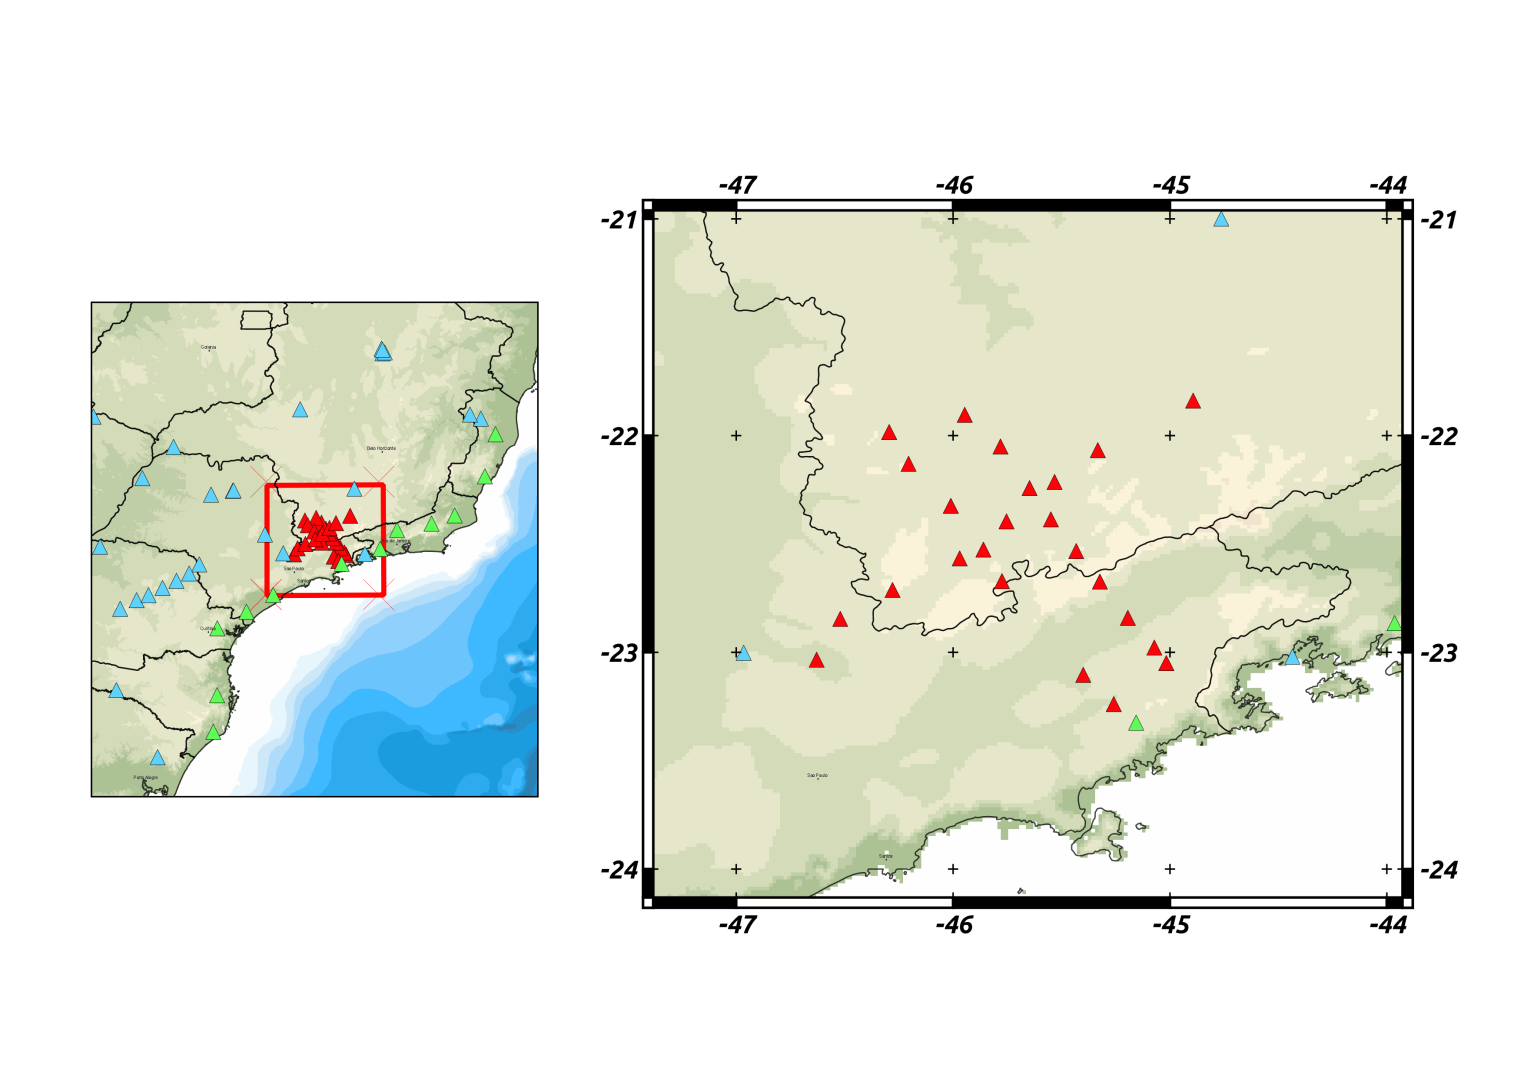
\includegraphics[scale=0.4]{mapa_das_estacoes_simosgraficas_instaladas.png}
\caption{Mapa das estações sismográficas instaladas (triângulos vermelhos). Os outros triângulos são estações da Rede Sismográfica Brasileira.}
\label{map_loc}
\end{figure}

O período de operação das estações foi distinto para os perfis. Os dois perfis perpendiculares à costa foram instalados no meio do ano de 2012 e o perfil paralelo no final de 2012. As estações ficaram em fucionamento até o final do ano de 2013 registrando o movimento do terreno de maneira contínua. 

O produto do deslocamento das partículas do meio registrado pelo sismógrafo, através de sensores verticais e horizontais em três componentes, pode ser visto na Figura \ref{simograma}. Esse registro da variação da amplitude em uma série temporal é chamado de sismograma. 

\begin{figure}[!ht]
\centering
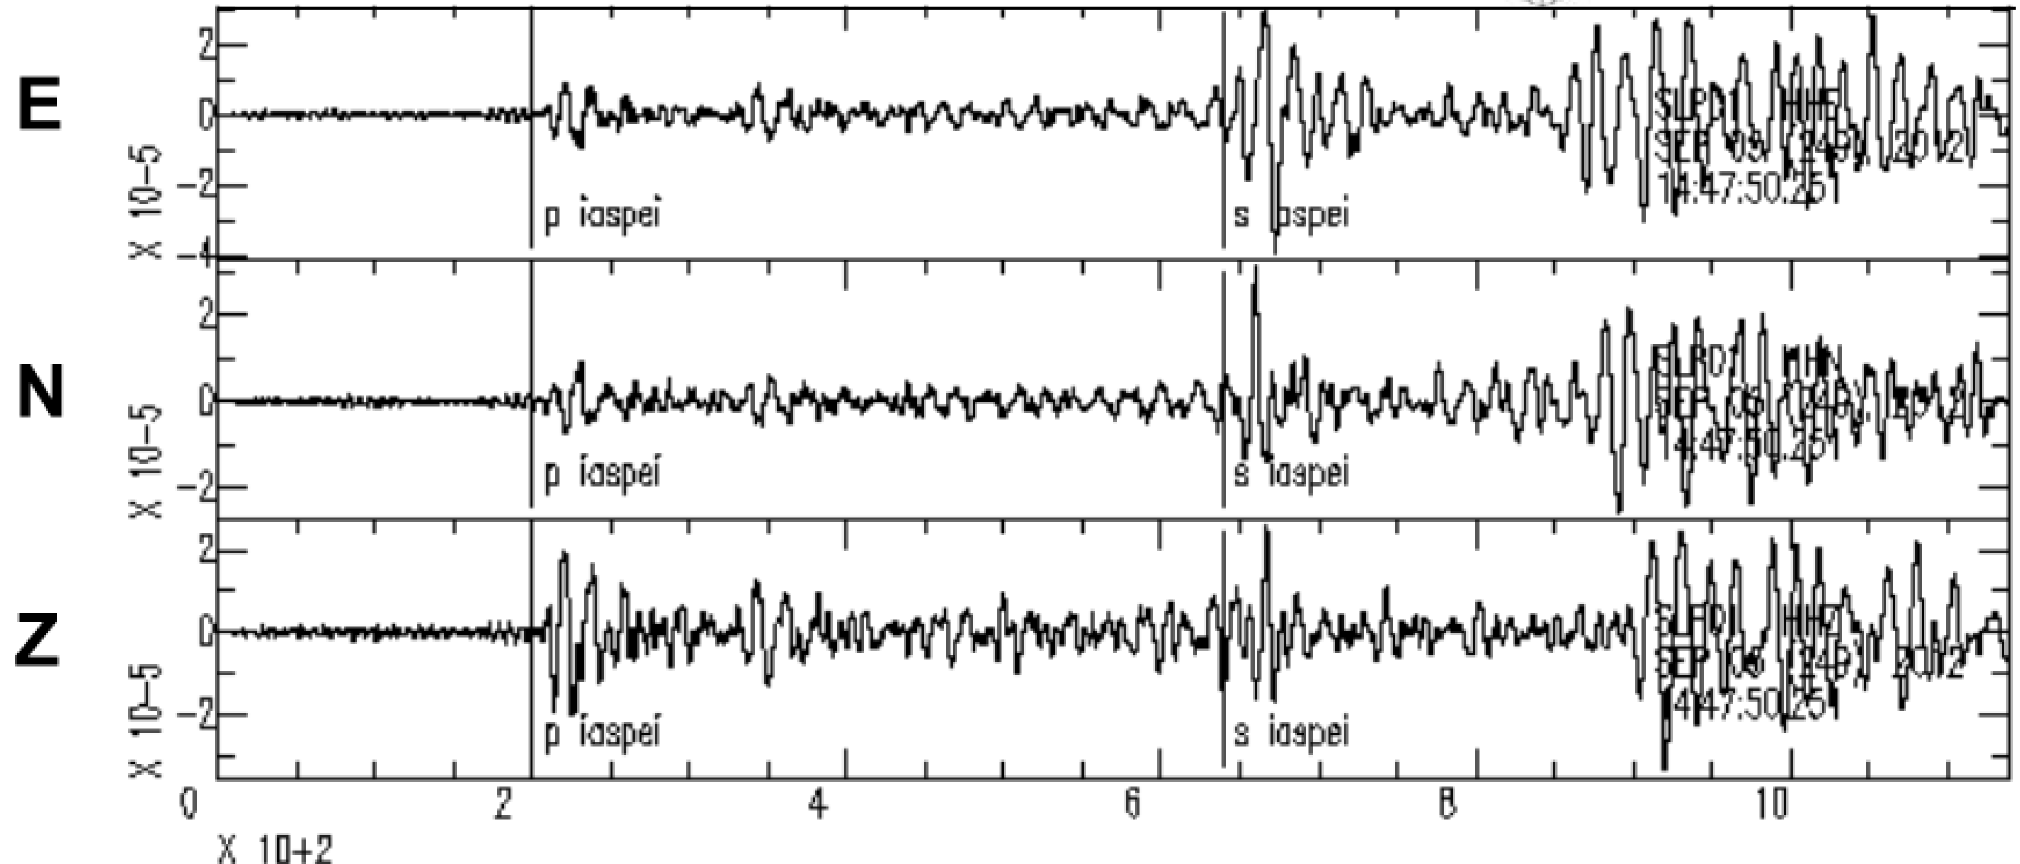
\includegraphics[scale=0.6]{sismograma.png}
\caption{Sismograma mostrandos as três componentes do deslocamento do terreno.}
\label{simograma}
\end{figure}

O sismograma é gerado pela perturbação do meio pelas ondas  mecânicas que se propagam no interior da Terra. Essas ondas  tem velocidades variando em função dos parâmetros elásticos do meio e da densidade. E estes variam pela mineralogia e condições de pressão e temperatura do meio atravessado. As ondas mecânicas são divididas em ondas de corpo e de superfície. As ondas de corpo estão categorizadas em dois tipos: as ondas P, longitudinal, e as ondas S, transversais. A onda P é mais rapida e que consegue se propagar em todos os meios, tem velocidade entre 4 e 7 km$/$s na crosta terrestre e em torno de 8 km$/$s no manto superior. As ondas S tem velocidade menor do que a onda P, em torno de 3 a 4 km$/$s na crosta.

Para produzir esta análise sobre a estrutura da região de estudo utilizou-se de um conjunto de dados com eventos sísmicos registrados. O número de eventos utilizados no processamento varia devido ao nível de sinal-ruído da forma da onda, pois há uma necessidade de visualização clara da chegada da onda P, como pode ser constatado na Figura \ref{simograma} .

\section{Tratamento dos Dados}

\subsection{Função do Receptor}

Para assegurar a confiabilidade do processamento é necessário um tratamento preliminar dos sinais brutos. Utilizou-se eventos catalogados na rede IRIS para uma identificação automática nestes sinais. Alguns pré-requisitos foram utilizados para a escolha dos eventos, como:

\begin{enumerate}
\item Distância Epicentral;
\item Magnitude;
\end{enumerate}

Sismos próximos, com distância menor que 20 graus da estação estudada, geram ondas com incidência oblíqua e esse tipo de dado deve ser utilizado com cuidado. Em sismos com distâncias maiores que 95 graus as ondas P não chegam na estação devido a inversão de velocidade no limite manto-núcleo, diminuição da velocidade da onda P entre o manto e o núcleo, e não é observada a onda P direta. Por isso a distância epicentral é tida como ideal entre 20 e 95 graus, como é observado na Figura \ref{mapa_eventos}. Devido grande parte dos sismos serem oriundos da Cordilheira dos Andes,como é visto na Figura \ref{teste_tempo}, também utilizou-se dados comn distância menor que 20 graus. A magnitude do sismo é importante para a propagação da onda, eventos com pequena magnitude não tem energia suficiente para gerar energia suficiente para gerar um sinal claro no sismograma.

\begin{figure}[!ht]
\centering
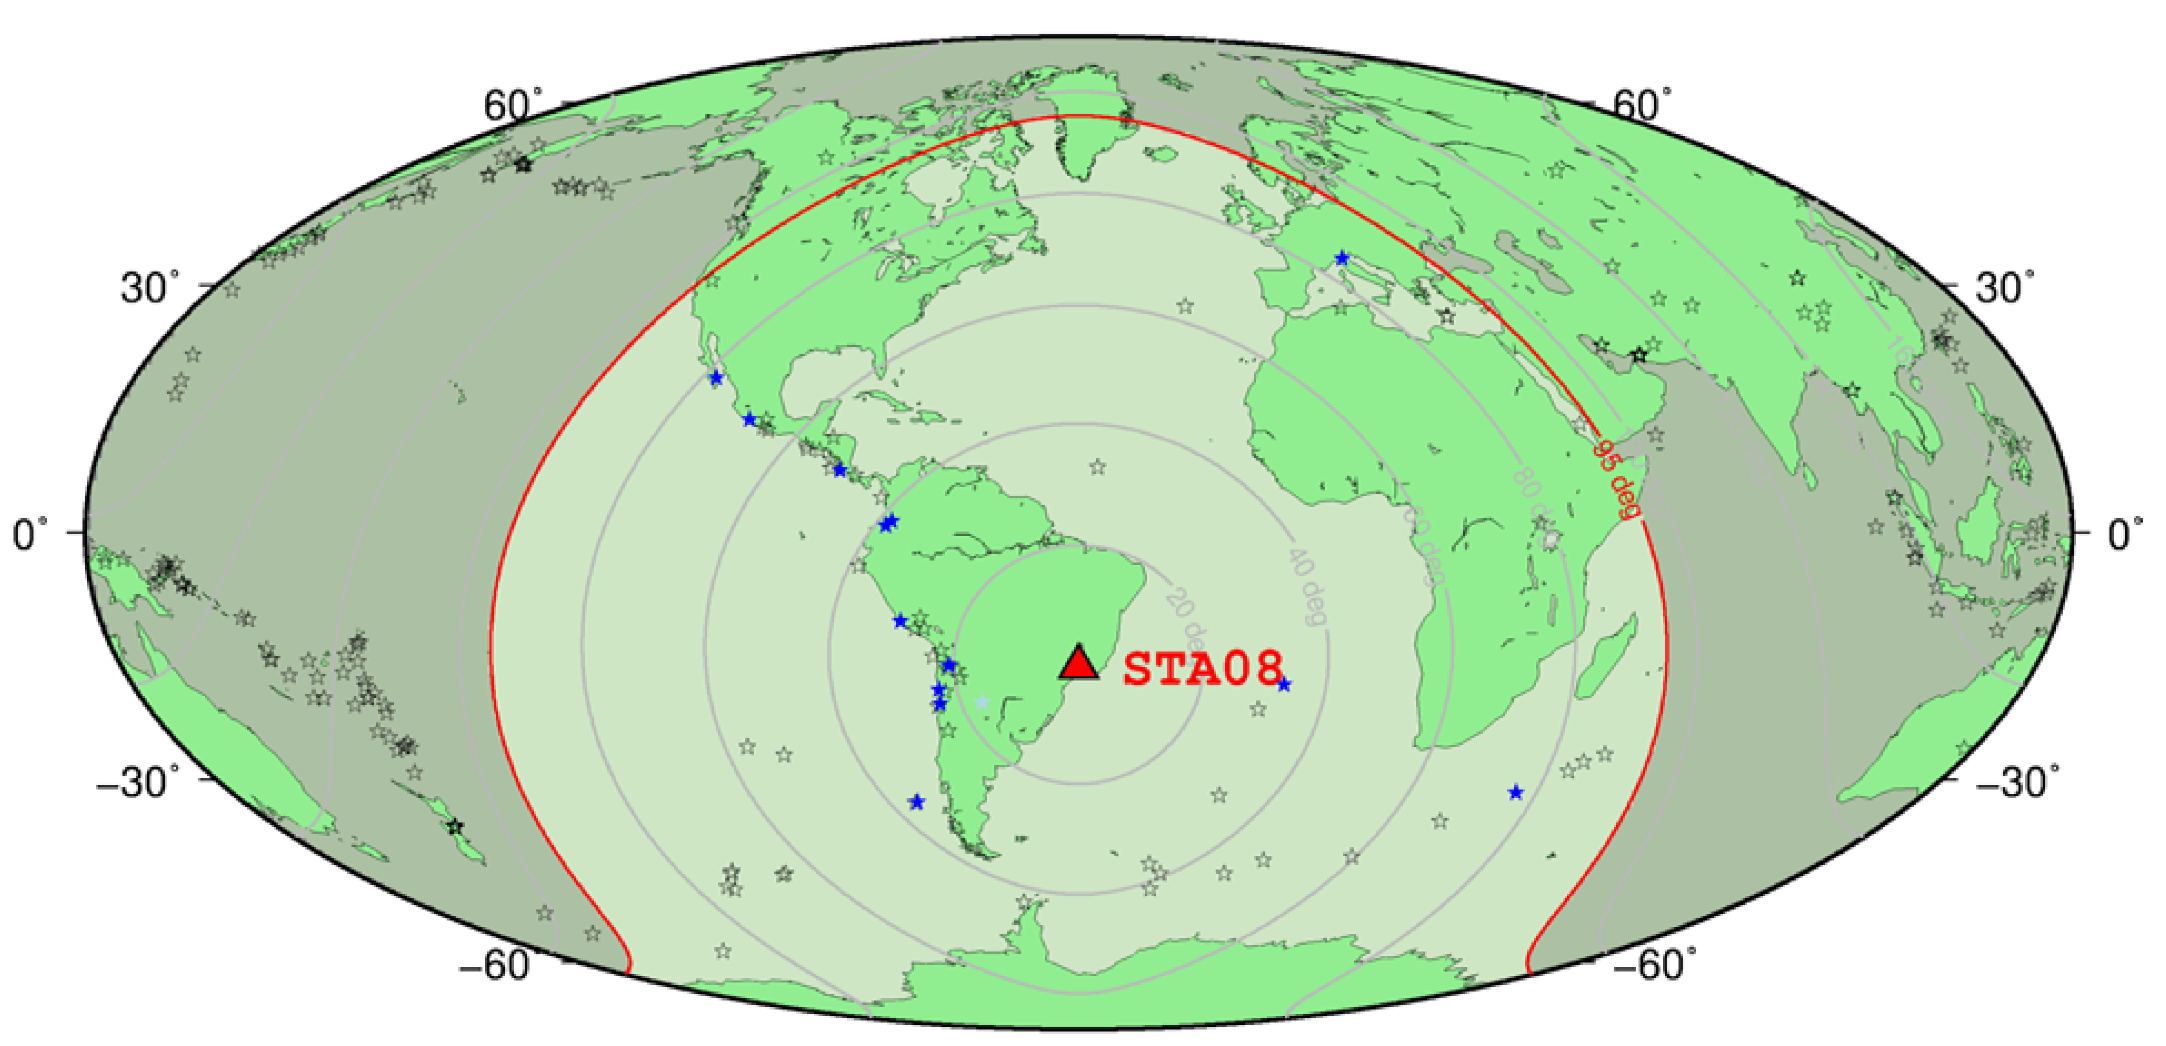
\includegraphics[scale=0.6]{mapa_de_eventos.png}
\caption{Mapa dos eventos (estrelas) registrados na estação STA08. O limite de 95 graus está indicada em vermelho. Estrelas azuls mostram os eventos com dados de qualidade que são usadas no calculo das Funçoes do Receptor}
\label{mapa_eventos}
\end{figure}


Subsequentemente um janelamento do registro em 5 segundos antes e 10 segundos depois da chegada da onda P, esta é calculada pelo modelo de velocidade da Terra  IASPEI91 \citep{kennet_iaspei_1991}. Após a discriminação e o janelamento do sinal, examina-se visualmente cada registro para certificar que todos os eventos selecionados tem um nível de sinal-ruído bom, como na Figura \ref{simograma} . 

Logo após removeu-se a média e tendência linear dos dados. Aplicou-se um filtro passa-alta com freqüência de corte de 0.1 Hz para eventos com distância entre 20 e 95 graus e de 2 Hz para eventos próximos (<20). Os dados originais com amostragens a cada 0,01 segundos (100 Hz) são interpolados para gerar dados com amostragens cada 0,025 segundas (40 Hz), porque a informação de alta freqüência não é relevante nesse tipo de análise.

\subsection{Dispersão de Ondas de Superfície}